\taskpic{ Металлическая звезда включена в сеть, как показано на
  рисунке. Сопротивление ребра $AC$ равно нулю, сопротивление ребра
  $BC$ равно $3R$, сопротивления остальных рёбер равны $R$. Найдите
  мощность, выделяющуюся по всей звезде. }
{
  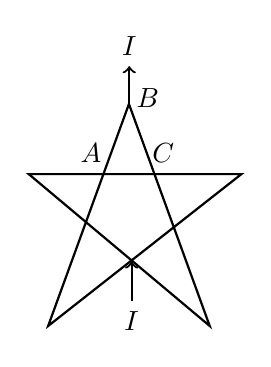
\begin{tikzpicture}
    \draw[thick] (0,0) -- ++(70:3cm) --++(-70:3cm) --++(140:3cm) --
    ++(0:2.7cm) --cycle;
    \draw (0.8,2.2) node[left] {$A$};
    \draw (1.2,2.2) node[right] {$C$};
    \draw (1,2.9) node[right] {$B$};
    \draw[thick,->] (1.03,2.8) -- ++(0,0.5) node[above] {$I$};
    \draw[thick,->] (1.06,0.32) node[below] {$I$} -- ++(0,0.5);
  \end{tikzpicture}
}
% НГУ, 3.90
